\documentclass[11pt]{article}
\usepackage[margin=18mm,headheight=22pt]{geometry}
\usepackage{amsmath}
\usepackage{fontspec}
\usepackage{unicode-math}
\setmainfont{NewCM10}[Extension=.otf,UprightFont=*-Book,BoldFont=*-Bold,ItalicFont=*-BookItalic,BoldItalicFont=*-BoldItalic]
\setsansfont{NewCMSans10}[Extension=.otf,UprightFont=*-Book,BoldFont=*-Bold,ItalicFont=*-BookOblique,BoldItalicFont=*-BoldOblique]
\setmathfont{NewCMMath-Book.otf}
\usepackage{xcolor}
\definecolor{FAUblue}{HTML}{04316A}
\definecolor{Paperblue}{HTML}{EEF2F7}
\definecolor{EEIgold}{HTML}{CC9C42}
\usepackage{etoolbox,enumitem,booktabs,tabularx,array,needspace,microtype}
\usepackage[most]{tcolorbox}
\usepackage{titlesec,fancyhdr}
\usepackage[hidelinks]{hyperref}
\usepackage{draftwatermark}
\SetWatermarkText{Made by Thanate Amornjiraporn (Focus)}
\SetWatermarkColor{black!7}\SetWatermarkFontSize{30pt}\SetWatermarkAngle{45}
\setlength{\parindent}{0pt}
\setlength{\parskip}{5pt}
\setlist{itemsep=2pt,topsep=3pt,leftmargin=1.6em,beginpenalty=10000,endpenalty=10000}
\raggedbottom
\clubpenalty=10000 \widowpenalty=10000 \displaywidowpenalty=10000 \interlinepenalty=10000
\setcounter{secnumdepth}{0}
\setcounter{tocdepth}{1}
\pagestyle{fancy}\fancyhf{}
\fancyhead[L]{\small\sffamily\color{FAUblue} From Fundamentals to AI Apocalypse · EEI · Exercise 3}
\fancyhead[R]{\small\sffamily Exercise 3: Worked solutions}
\fancyfoot[C]{\small\thepage}
\titleformat{\section}{\Large\bfseries\sffamily\color{FAUblue}}{}{0pt}{}
\titleformat{\subsection}{\large\bfseries\sffamily\color{FAUblue}}{}{0pt}{}
\titlespacing*{\section}{0pt}{16pt}{6pt}
\preto\section{\Needspace{8\baselineskip}}
\preto\subsection{\Needspace{6\baselineskip}}
\newtcolorbox{equationcard}[1]{colback=Paperblue,colframe=Paperblue,boxrule=0pt,arc=0pt,left=10pt,right=10pt,top=6pt,bottom=6pt,title={#1},fonttitle=\small\bfseries\sffamily,coltitle=FAUblue,before skip=8pt,after skip=8pt}
\newtcolorbox{workedbox}[1]{colback=white,colframe=EEIgold,boxrule=0pt,leftrule=3pt,arc=0pt,left=10pt,top=4pt,bottom=4pt,title={#1},fonttitle=\small\bfseries\sffamily,coltitle=FAUblue,attach title to upper={\par},before skip=8pt,after skip=8pt}
\newtcolorbox{recallbox}[1]{colback=white,colframe=FAUblue,boxrule=0pt,leftrule=3pt,arc=0pt,left=10pt,top=4pt,bottom=4pt,title={#1},fonttitle=\small\bfseries\sffamily,coltitle=FAUblue,attach title to upper={\par},before skip=8pt,after skip=8pt}
\usepackage{environ}
\newsavebox\measurebox
% Typeset the section once invisibly to measure it; start a new page if it will not fit in what is left.
\makeatletter
\newif\ifkeep@measuring
\NewEnviron{keepsection}{%
  \ifkeep@measuring \BODY \else
    \edef\keep@sec{\the\value{section}}\edef\keep@sub{\the\value{subsection}}%
    \setbox\measurebox\vbox{\hsize\linewidth\keep@measuringtrue\def\Needspace##1{}\BODY}%
    \setcounter{section}{\keep@sec}\setcounter{subsection}{\keep@sub}%
    \dimen2=\ht\measurebox \advance\dimen2\dp\measurebox
    \dimen@=\textheight
    \ifdim\pagegoal<\maxdimen
      \dimen@=\pagegoal \advance\dimen@-\pagetotal
      \ifdim\dimen2>\dimen@ \clearpage \dimen@=\textheight \fi
    \fi
    % if it fits, nothing inside may force an early break
    \ifdim\dimen2>\dimen@ \BODY \else \begingroup\def\Needspace##1{}\BODY\endgroup \fi
  \fi}
\makeatother
\newtcolorbox{notebox}{colback=Paperblue,colframe=Paperblue,boxrule=0pt,arc=0pt,left=8pt,right=8pt,top=4pt,bottom=4pt,before skip=6pt,after skip=6pt}
\newtcolorbox{plainbox}{colback=white,colframe=FAUblue,boxrule=0pt,leftrule=3pt,arc=0pt,left=10pt,right=8pt,top=4pt,bottom=4pt,before skip=6pt,after skip=8pt}
\usetikzlibrary{arrows.meta}
\title{\sffamily\bfseries\color{FAUblue}Exercise 3: Worked solutions}
\author{Electrical Engineering I \ensuremath{\cdot} Module 92315 \ensuremath{\cdot} Exercise 3\\[2pt]\small From Fundamentals to AI Apocalypse · personal study guide}
\date{}
\begin{document}
\maketitle
\begingroup\footnotesize\setlength{\parskip}{0pt}\tableofcontents\endgroup
\clearpage

\Needspace{8\baselineskip}
{\large Try each part before opening the answer. We use symmetry to choose Gaussian surfaces, then split the capacitor into the dielectric core and the air annulus.}


\begin{keepsection}
\Needspace{9\baselineskip}
\section{Task 7: Electric field of a uniformly charged sphere}

\Needspace{6\baselineskip}
A spherical volume charge has density \textit{ρ}\textsubscript{0} for 0 \ensuremath{\leq} \textit{r} \ensuremath{\leq} \textit{a} and zero outside. Its centre is the origin. Find the field everywhere in vacuum, where \textit{D} = \textit{ε}\textsubscript{0}\textit{E}.

\Needspace{9\baselineskip}
\textbf{Connected topic:} Gauss’s law (§1.10) turns spherical symmetry into a flux equation on a concentric sphere.

\Needspace{14\baselineskip}
\begin{center}
\begin{minipage}[t]{0.950\linewidth}\centering
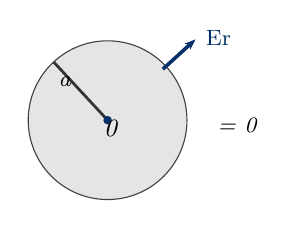
\begin{tikzpicture}
\filldraw[draw=black!75,fill=black!10] (2.016,-1.512) circle (1.008);
\draw[black!80,line width=1pt] (2.016,-1.512) -- (1.332,-0.774);
\fill[FAUblue] (2.016,-1.512) circle (0.054);
\draw[-{Stealth[length=4pt]},FAUblue,line width=1.3pt] (2.718,-0.864) -- (3.132,-0.486);
\node[,inner sep=1pt,font=\footnotesize] at (1.476,-1.026) {\textit{a}};
\node[,inner sep=1pt,font=\small] at (2.016,-1.620) {\textit{ρ0}};
\node[anchor=west,inner sep=1pt,font=\footnotesize] at (3.186,-1.584) {\textit{ρ = 0}};
\node[anchor=west,text=FAUblue,inner sep=1pt,font=\footnotesize] at (3.222,-0.468) {Er};
\end{tikzpicture}\par\smallskip{\small\raggedright \textbf{Enclosed charge depends on the Gaussian radius.} Inside the material only the smaller sphere contributes; outside it, the entire charged sphere is enclosed.\par}\end{minipage}
\end{center}

\begin{keepsection}
\Needspace{7\baselineskip}
\subsection{7: Field inside and outside}

\Needspace{4\baselineskip}
Try first: choose a concentric spherical Gaussian surface of radius \textit{r}, and find its enclosed charge separately for \textit{r} \ensuremath{\leq} \textit{a} and \textit{r} \ensuremath{>} \textit{a}.

\nopagebreak[4]{\small\itshape Answers: see “Task 7: Electric field of a uniformly charged sphere” under Answers at the end.}
\end{keepsection}
\end{keepsection}

\begin{keepsection}
\Needspace{11\baselineskip}
\section{Task 8: Parallel plates with a dielectric cylinder}

\Needspace{8\baselineskip}
Two circular metal plates have radius \textit{a}\textsubscript{2} and separation \textit{h}. A concentric dielectric cylinder of radius \textit{a}\textsubscript{1} fills the gap between the plates; the annular region from \textit{a}\textsubscript{1} to \textit{a}\textsubscript{2} is air. The source assumes uniform axial fields in both regions and neglects fringing at the plate edge.

\Needspace{10\baselineskip}
\textbf{Connected topics:} Capacitance (§1.13) relates charge and voltage; field energy (§1.14) gives the stored energy. Interpret \textit{ε}\textsubscript{1} as the absolute permittivity of the cylinder, as distinguished from \textit{ε}\textsubscript{0} for air in the figure.

\Needspace{14\baselineskip}
\begin{center}
\begin{minipage}[t]{0.950\linewidth}\centering
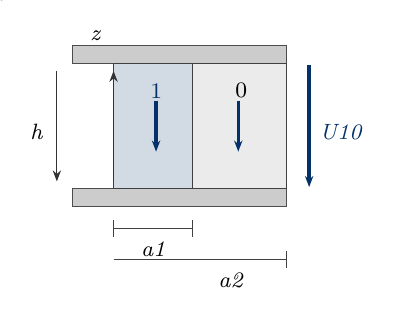
\begin{tikzpicture}
\filldraw[draw=black!70,fill=black!20] (0.954,-0.540) rectangle (3.672,-0.774);
\filldraw[draw=black!70,fill=black!20] (0.954,-2.358) rectangle (3.672,-2.592);
\filldraw[draw=black!75,fill=FAUblue!18] (1.476,-0.774) rectangle (2.484,-2.358);
\filldraw[draw=black!75,fill=black!8] (2.484,-0.774) rectangle (3.672,-2.358);
\draw[-{Stealth[length=4pt]},black!80] (1.476,-2.268) -- (1.476,-0.864);
\draw[-{Stealth[length=4pt]},black!80] (0.756,-0.864) -- (0.756,-2.268);
\node[anchor=east,inner sep=1pt,font=\footnotesize] at (0.630,-1.638) {\textit{h}};
\draw[-{Stealth[length=4pt]},FAUblue,line width=1.2pt] (2.016,-1.242) -- (2.016,-1.890);
\draw[-{Stealth[length=4pt]},FAUblue,line width=1.2pt] (3.060,-1.242) -- (3.060,-1.890);
\draw[-{Stealth[length=4pt]},FAUblue,line width=1.2pt] (3.960,-0.792) -- (3.960,-2.340);
\node[anchor=east,inner sep=1pt,font=\footnotesize] at (1.368,-0.414) {\textit{z}};
\node[text=FAUblue,inner sep=1pt,font=\footnotesize] at (1.980,-1.116) {ε1};
\node[,inner sep=1pt,font=\footnotesize] at (3.060,-1.116) {ε0};
\node[anchor=west,text=FAUblue,inner sep=1pt,font=\footnotesize] at (4.050,-1.638) {\textit{U10}};
\draw[black!75] (1.476,-2.754) -- (1.476,-2.970);
\draw[black!75] (2.484,-2.754) -- (2.484,-2.970);
\draw[black!75] (3.672,-3.150) -- (3.672,-3.366);
\draw[black!75] (1.476,-2.862) -- (2.484,-2.862);
\draw[black!75] (1.476,-3.258) -- (3.672,-3.258);
\node[,inner sep=1pt,font=\footnotesize] at (1.980,-3.132) {\textit{a1}};
\node[,inner sep=1pt,font=\footnotesize] at (2.970,-3.528) {\textit{a2}};
\end{tikzpicture}\par\smallskip{\small\raggedright \textbf{Two materials share the same plate voltage.} The axial field is uniform within each region; the radial material boundary separates the dielectric core from the air annulus.\par}\end{minipage}
\end{center}

The source labels the applied voltage \textit{U}\textsubscript{10} with an arrow from the upper plate to the lower one. Use the standard convention \textit{U}\textsubscript{10} = \textit{V}\textsubscript{1} \ensuremath{-} \textit{V}\textsubscript{0}, upper minus lower; for positive \textit{U}\textsubscript{10}, the field points down, along \ensuremath{-}\textit{e}\textsubscript{z}.

\begin{keepsection}
\Needspace{7\baselineskip}
\subsection{8a: Field between the plates}

\Needspace{4\baselineskip}
Try first: relate the potential difference to the axial field, then use tangential-field continuity at the cylindrical material boundary.

\nopagebreak[4]{\small\itshape Answers: see “Task 8: Parallel plates with a dielectric cylinder” under Answers at the end.}
\end{keepsection}

\begin{keepsection}
\Needspace{7\baselineskip}
\subsection{8b: Charge on the underside of the upper plate}

\Needspace{4\baselineskip}
Try first: find the free surface charge density in each patch from D = εE and the normal pointing from the upper conductor into the gap.

\nopagebreak[4]{\small\itshape Answers: see “Task 8: Parallel plates with a dielectric cylinder” under Answers at the end.}
\end{keepsection}

\begin{keepsection}
\Needspace{6\baselineskip}
\subsection{8c: Capacitance}

\Needspace{3\baselineskip}
Try first: divide the upper-plate charge by the applied voltage.

\nopagebreak[4]{\small\itshape Answers: see “Task 8: Parallel plates with a dielectric cylinder” under Answers at the end.}
\end{keepsection}

\begin{keepsection}
\Needspace{7\baselineskip}
\subsection{8d: Energy change when the dielectric is removed}

\Needspace{4\baselineskip}
Try first: compute the initial and final capacitances, then compare their field energies at the same fixed voltage.

\nopagebreak[4]{\small\itshape Answers: see “Task 8: Parallel plates with a dielectric cylinder” under Answers at the end.}
\end{keepsection}
\end{keepsection}


\clearpage
\section{Answers}
\begin{keepsection}\subsection{Task 7: Electric field of a uniformly charged sphere}

\begin{workedbox}{7 \ensuremath{\cdot} Gauss’s law in the two regions}
\Needspace{17\baselineskip}
\begin{enumerate}
\item \Needspace{5\baselineskip}
Spherical symmetry makes the field radial and equally strong everywhere on a concentric Gaussian sphere. Its area is 4π\textit{r}\textsuperscript{2}, so the flux law reduces to:

\Needspace{4\baselineskip}
\begin{equation*}\oiint \, {D}\, \cdot \, \mathrm{d}{A}\, =\, {D}_{\mathrm{r}}({r})\, 4π{r}^{2}\, =\, {Q}_{\text{enc}}({r})\end{equation*}

Since \textit{D} = \textit{ε}\textsubscript{0}\textit{E}, solving this gives \textit{E}\textsubscript{r} once we know the enclosed charge.
\item \Needspace{5\baselineskip}
For 0 \ensuremath{<} \textit{r} \ensuremath{\leq} \textit{a}, the Gaussian sphere contains only a smaller volume of the uniform density. The spherical volume is 4π\textit{r}\textsuperscript{3}/3:

\begin{equation*}{Q}_{\text{enc}}({r})\, =\, {ρ}_{0}\dfrac{4π{r}^{3}}{3}\end{equation*}
\item \Needspace{4\baselineskip}
Substitute that enclosed charge into Gauss’s law and divide by 4π\textit{ε}\textsubscript{0}\textit{r}\textsuperscript{2}:

\begin{equation*}{E}_{\mathrm{r}}({r})\, =\, \dfrac{{Q}_{\text{enc}}}{4π{ε}_{0}{r}^{2}}\, =\, \dfrac{{ρ}_{0}{r}}{3{ε}_{0}},\, \quad \, 0\, \leq \, {r}\, \leq \, {a}\end{equation*}
\item \Needspace{5\baselineskip}
For \textit{r} \ensuremath{>} \textit{a}, the Gaussian sphere encloses all the charge, whose volume is the full sphere of radius \textit{a}:

\begin{equation*}{Q}_{\text{total}}\, =\, {ρ}_{0}\dfrac{4π{a}^{3}}{3};\, \quad \, {E}_{\mathrm{r}}({r})\, =\, \dfrac{{ρ}_{0}{a}^{3}}{3{ε}_{0}{r}^{2}},\, \quad \, {r}\, >\, {a}\end{equation*}
\item \Needspace{4\baselineskip}
\textbf{Result:} for the positive density shown, the vector field points radially outward. Inside:

\Needspace{4\baselineskip}
\begin{equation*}{E}({r})\, =\, \dfrac{{ρ}_{0}{r}}{3{ε}_{0}}{e}_{\mathrm{r}},\, \quad \, 0\, \leq \, {r}\, \leq \, {a}\end{equation*}

\Needspace{4\baselineskip}
Outside, all charge is enclosed:

\Needspace{4\baselineskip}
\begin{equation*}{E}({r})\, =\, \dfrac{{ρ}_{0}{a}^{3}}{3{ε}_{0}{r}^{2}}{e}_{\mathrm{r}},\, \quad \, {r}\, >\, {a}\end{equation*}

\Needspace{6\baselineskip}
At the origin, \textit{E} = 0; negative \textit{ρ}\textsubscript{0} reverses the radial direction.

\textbf{Check:} both formulas give \textit{E}(\textit{a}) = \textit{ρ}\textsubscript{0}\textit{a}/(3\textit{ε}\textsubscript{0}), so the field is continuous at the surface. Far away it falls as 1/\textit{r}\textsuperscript{2}, as if the total charge were concentrated at the centre. With SI inputs, E is in N/C.
\end{enumerate}
\end{workedbox}

\end{keepsection}
\begin{keepsection}\subsection{Task 8: Parallel plates with a dielectric cylinder}

\begin{workedbox}{8a \ensuremath{\cdot} One voltage, two regions}
\Needspace{14\baselineskip}
\begin{enumerate}
\item \Needspace{5\baselineskip}
The field is uniform and axial in each region. Moving from the lower plate at z = 0 to the upper plate at z = h gives the upper-minus-lower potential:

\begin{equation*}{U}_{10}\, =\, {V}_{1}\, -\, {V}_{0}\, =\, -\int_{0}^{\mathrm{h}} \, {E}_{\mathrm{z}}\, \mathrm{d}{z}\end{equation*}
\item \Needspace{5\baselineskip}
The radial boundary at ρ = \textit{a}\textsubscript{1} is parallel to the z-directed field. Its tangential field component is continuous, so the assumed axial components agree:

\begin{equation*}{E}_{1}\, =\, {E}_{2}\, =\, {E}_{\mathrm{z}}\end{equation*}
\item \Needspace{5\baselineskip}
Because each field is uniform over the gap, the integral is \textit{E}\textsubscript{z}\textit{h}. Solve for the common component:

\begin{equation*}{E}_{1}\, =\, {E}_{2}\, =\, -\dfrac{{U}_{10}}{{h}}\end{equation*}
\item \Needspace{4\baselineskip}
\textbf{Result:} in the requested gap (not inside the metal), the field is the same everywhere:

\Needspace{5\baselineskip}
\begin{equation*}{E}\, =\, -\dfrac{{U}_{10}}{{h}}\, {e}_{{z}},\, \quad \, 0\, \leq \, ρ\, \leq \, {a}_{2},\, \quad \, 0\, <\, {z}\, <\, {h}\end{equation*}

\Needspace{6\baselineskip}
The same field applies on both sides of ρ = \textit{a}\textsubscript{1} under the uniform-field approximation. The material changes D, not this tangential E.

\textbf{Check:} E has units V/m. For positive upper-minus-lower voltage, potential decreases in the +z direction, so E points downward.
\end{enumerate}
\end{workedbox}

\end{keepsection}
\begin{keepsection}\subsection{Task 8: Parallel plates with a dielectric cylinder}

\begin{workedbox}{8b \ensuremath{\cdot} Add the two material patches}
\Needspace{14\baselineskip}
\begin{enumerate}
\item The outward normal from the lower face of the upper metal plate into the gap is \ensuremath{-}\textit{e}\textsubscript{z}. The conductor boundary relation gives free surface charge density σ\textsubscript{f} = \textit{D} \ensuremath{\cdot} n. Since \textit{E} = \ensuremath{-}(\textit{U}\textsubscript{10}/\textit{h})\textit{e}\textsubscript{z}, each patch has positive σ for positive U\textsubscript{10}.
\item \Needspace{4\baselineskip}
Over the dielectric circle, \textit{D} = \textit{ε}\textsubscript{1}\textit{E}; its area is π\textit{a}\textsubscript{1}\textsuperscript{2}:

\begin{equation*}{Q}_{\text{core}}\, =\, σ_{1}π{a}_{1}^{2}\, =\, \dfrac{{ε}_{1}{U}_{10}}{{h}}π{a}_{1}^{2}\end{equation*}
\item \Needspace{4\baselineskip}
Over the air annulus, \textit{D} = \textit{ε}\textsubscript{0}\textit{E}; its area is the whole plate disk minus the core disk:

\begin{equation*}{Q}_{\text{air}}\, =\, σ_{2}π({a}_{2}^{2}\, -\, {a}_{1}^{2})\, =\, \dfrac{{ε}_{0}{U}_{10}}{{h}}π({a}_{2}^{2}\, -\, {a}_{1}^{2})\end{equation*}
\item \Needspace{4\baselineskip}
Add the two disjoint patches on the same metal face:

\Needspace{5\baselineskip}
\begin{equation*}{Q}\, =\, {Q}_{\text{core}}\, +\, {Q}_{\text{air}}\, =\, \dfrac{{πU}_{10}}{{h}}[{ε}_{1}{a}_{1}^{2}\, +\, {ε}_{0}({a}_{2}^{2}\, -\, {a}_{1}^{2})]\end{equation*}

\Needspace{6\baselineskip}
\textbf{Result:} this is the charge on the underside of the upper plate. For positive U\textsubscript{10} it is positive; the lower plate carries the opposite charge.

\textbf{Check:} each term has permittivity \ensuremath{\times} voltage \ensuremath{\times} area / length, which is coulombs. If a\textsubscript{1} = 0 the full plate is air; if a\textsubscript{1} = a\textsubscript{2} it is fully filled by the dielectric.
\end{enumerate}
\end{workedbox}

\end{keepsection}
\begin{keepsection}\subsection{Task 8: Parallel plates with a dielectric cylinder}

\begin{workedbox}{8c \ensuremath{\cdot} Charge-to-voltage ratio}
\Needspace{7\baselineskip}
\begin{enumerate}
\item \Needspace{4\baselineskip}
Capacitance is defined by \textit{C} = \textit{Q}/\textit{U}. Divide the expression from 8b by \textit{U}\textsubscript{10}:

\begin{equation*}{C}\, =\, \dfrac{{π}}{{h}}[{ε}_{1}{a}_{1}^{2}\, +\, {ε}_{0}({a}_{2}^{2}\, -\, {a}_{1}^{2})]\end{equation*}
\item \Needspace{6\baselineskip}
\textbf{Result:} this is the capacitance under the stated uniform-field model. The two regions behave like capacitors in parallel because they span the same voltage and their charges add.

\textbf{Check:} it equals the sum of area/permittivity contributions divided by h; capacitance has units farads.
\end{enumerate}
\end{workedbox}

\end{keepsection}
\begin{keepsection}\subsection{Task 8: Parallel plates with a dielectric cylinder}

\begin{workedbox}{8d \ensuremath{\cdot} Fixed-voltage energy change}
\Needspace{18\baselineskip}
\begin{enumerate}
\item \Needspace{4\baselineskip}
Initially the capacitance is the value from 8c. After removal, the whole plate area is air:

\begin{equation*}{C}_{\mathrm{i}}\, =\, \dfrac{{π}}{{h}}[{ε}_{1}{a}_{1}^{2}\, +\, {ε}_{0}({a}_{2}^{2}\, -\, {a}_{1}^{2})];\, \quad \, {C}_{\mathrm{f}}\, =\, \dfrac{{ε}_{0}π{a}_{2}^{2}}{{h}}\end{equation*}
\item \Needspace{5\baselineskip}
With voltage held fixed, stored field energy is \textit{W} = \ensuremath{\tfrac12}\textit{C U}\textsuperscript{2}. Subtract the initial energy from the final energy:

\begin{equation*}Δ{W}_{\text{field}}\, =\, \tfrac{1}{2}({C}_{\mathrm{f}}\, -\, {C}_{\mathrm{i}}){U}_{10}^{2}\end{equation*}
\item \Needspace{4\baselineskip}
The air-region terms cancel, leaving the contribution from the removed core:

\begin{equation*}Δ{W}_{\text{field}}\, =\, -\dfrac{{πa}_{1}^{2}({ε}_{1}\, -\, {ε}_{0})}{2{h}}{U}_{10}^{2}\end{equation*}
\item \Needspace{7\baselineskip}
Follow the energy that leaves. With \textit{U}\textsubscript{10} fixed, the plate charge changes by Δ\textit{Q} = (\textit{C}\textsubscript{f} \ensuremath{-} \textit{C}\textsubscript{i})\textit{U}\textsubscript{10} \ensuremath{<} 0, so charge flows back into the source. The energy the source delivers is \textit{W}\textsubscript{source} = \textit{U}\textsubscript{10}Δ\textit{Q} = 2Δ\textit{W}\textsubscript{field}, a negative number: the source takes energy back. Whoever pulls the core out supplies the difference:

\begin{equation*}{W}_{\text{mech}}\, =\, Δ{W}_{\text{field}}\, -\, {W}_{\text{source}}\, =\, -Δ{W}_{\text{field}}\, =\, \dfrac{π{a}_{1}^{2}(ε_{1}\, -\, ε_{0})}{2{h}}{U}_{10}^{2}\end{equation*}
\item \Needspace{8\baselineskip}
\textbf{Result:} if \textit{ε}\textsubscript{1} \ensuremath{>} \textit{ε}\textsubscript{0}, the stored field energy decreases by this amount (Δ\textit{W}\textsubscript{field} \ensuremath{<} 0), measured in joules. Positive mechanical work of the same size is needed to pull the core out: at fixed voltage the field draws the dielectric into the gap, and the source takes back twice the field-energy drop.

\textbf{Check:} if the core is indistinguishable from air, ε\textsubscript{1} = ε\textsubscript{0}, the change is zero. The magnitude scales with the removed area and with voltage squared.
\end{enumerate}
\end{workedbox}

\end{keepsection}

\vfill{\small Personal worked-solution guide based on the supplied EEI Exercise 3 sheet, written in my own words; no exercise text or figures are reproduced. Not an official FAU publication; check course details against current material. Made by \textbf{Thanate Amornjiraporn (Focus)}.}

\end{document}
